%% Available online at https://www.overleaf.com/11445166drmnqzsywytj#/43230232/

\documentclass[11pt]{article}

\usepackage{booktabs}
\usepackage{homeworkpkg}
\usepackage{enumitem}
\usepackage[font=small,labelfont=bf]{caption}
\usepackage[bottom]{footmisc}

\newlength\dunder
\settowidth{\dunder}{\_}

\graphicspath{ {images/} }

%% Local Macros and packages: add any of your own definitions here.

\begin{document}

% Homework number, your name and NetID, and optionally, the names/NetIDs of anyone you collaborated with. If you did not collaborate with anybody, leave the last parameter empty.
\homework
    {2}
    {Nestor Alejandro Bermudez Sarmiento (nab6)}
    {Edward McEnrue (mcenrue2)}

We've decided to use Python for this assignment. The source code is provided with this report.\\

\section*{Part 1: CSP - Flow Free}

The following description is valid for both Part 1.1 and Part 1.2.\\

We are given the game Free Flow to model as a Constraint Satisfaction Problem (CSP). The definition of free flow is quite simple. Given a 2D grid, and $n$ colors, each color with 2 corresponding sources/nodes in the grid, and where each source/node gets placed in some seemingly random position on that grid, one must determine a pipe/path of coordinates between each color pair of sources/nodes, such that no two pipes/paths between color pair of sources/nodes share a coordinate, and all coordinates on the grid contain a part of a pipe/path, or a source/node. Also, for every coordinate of every path, each coordinate that isn't one of the sources must share \textbf{exactly} 2 sides with the same color. Finally, it turns out that there is only one solution per grid. A more formal definition of the environment yields the following.\\

We have $2n$ sources/nodes, where $n$ is the number of colors. Each of these $2n$ sources/nodes can be represented by a set of coordinates, $S$, with $s_i \in S$ having some $(y,x) \in M$, along with a value (we will define values in our domain discussion below). We also have a grid of coordinates, $M$, with number of rows $r$ and number of columns $c$. All $2n$ sources/nodes have a unique coordinate $(i,j) \in M$ where $0 \leq i \leq r$ and $0 \leq j \leq c$. From this environment definition, we still must define our CSP.\\




Any CSP has a state with variables $X_i$, values $v_i \in D$ domain; a goal test delimiting the set of constraints for the combination of $v_i$ for our $X_i$; and a solution, which is just a complete and consistent assignment of $v_i$ to $X_i$. Let us enumerate these components and their definition for the CSP on Free Flow with respect to our previous environment definition:



\begin{enumerate}
\item \textit{variables}: A variable $X_i$ is defined as a coordinate $(i, j) \in M$ and $(i, j) \not\in S$.
\item \textit{domain}: $n$ is the set of colors defined as part of our Free Flow input where $1 \leq ||n|| \leq (r*c)/2$ and each $c_i \in n$ we can represent as a number $1 \leq v_i \leq ||n||$. T is the set of block types where a block type can have open ends in the following ways: {(up, down): VE, (left, right): HO, (up, right): NE, (right, down): SE, (down, left): SW, (left, up): NW}. Every variable is assigned both a color and block type for its value.
\item \textit{constraints}:
There are multiple constraints. At a high level, let's consider the cardinal directions (up, down, left, right) to be neighbors of each variable. From this, we can define our constraints.

\begin{enumerate}
\item
If we have a neighbor that is a source, and that source is at an open end of the current variable, then the source must be the same color as our current variable, and that source must not have any other neighbors with the current variable's color.

\item
If we have a neighbor that isn't a source or empty, and that neighbor has an open end towards the current variable or the current variable has an open end towards that neighbor, then both the current variable and that neighbor must have the same color and they must both have an open end facing each other.

\item
For any square on the grid $M$ composed of four locations (variables), then those variables must not all have the same color. This global constraint can be restated to be a local constraint by saying each of the 4 squares that a variable can be a part of (assuming that variable isn't on an edge of the grid) must not contain 4 variables with the same color.

\end{enumerate}
\item \textit{Goal Test}
Since our constraints are consistent, then we actually only need to check that there is an assignment for every variable as this will produce the requisite paths between sources without zig zags as necessary.
\end{enumerate}

Now that we have formulated free flow as a CSP, we can define our backtracking algorithm, which we used for both part 1.1 and 1.2. As a base definition of our backtracking algorithm, we will use the one defined on Page 215, Figure 6.5 of the textbook. The definition that the book gives for this particular figure includes ordering of variables, values, and using inference.

If you were to remove the ordering of variables, values and the usage of inference, then the result is identical to what we used for our "dumb" solution as referred to by problem 1.1. In other words, no value or variable ordering, and no inference is used in our backtracking algorithm for our "dumb" solution. Variables and values are selected randomly. Once this "dumb" solution was implemented, we tested it on the 7x7 maze shown in figure 1. It was not able to complete this input, but it was able to complete the 5x5 test maze. This should be expected, since the performance of general backtracking on a general CSP is $O(m^n)$ where $m$ is the max amount of values per variable and $n$ is the number of variables. From this, we knew we would have to incorporate heuristics in order to solve the 7x7, 8x8, and 9x9 mazes in figures 1, 3, and 5 respectively.

\pagebreak
\subsection*{PART 1.1: Smaller Inputs: for Everyone}


Once we added our heuristics to our backtracking algorithm, we were able to achieve the desired solutions as shown in figures 1, 3, and 5. Likewise, we show the times for these solutions with the heuristics in table 1.

Our first heuristic is ordering variable selection by the most constrained variables first. This ultimately decreases the branching factor of the backtracking algorithm. The selection of the most constrained variable was performed in the same part of the backtracking algorithm as the random selection was. When most constrained variable selection was used, we would analyze all unassigned variables and count the amount of consistent values that variable had available. We would then select the variable with the smallest amount of consistent value assignments available. Our consistency was defined as checking if a value was not violating one of the aforementioned constraints.

The second heuristic is ordering value selection by the least constraining value first. Similar to most constrained variables first, least constraining value first yields less constraints for other variables thus increasing the likelihood of a solution being achieved for a particular branch. The selection of least constraining value was performed in the same part of the backtracking algorithm as the random ordering value selection was. When least constraining value is used, we would look at a value for a particular variable and sum up the total amount of values remaining in neighbors. We would do this for all possible values that can be assigned to that variable, and then we would select the value which which yields the largest sum. We also make use of most constraining value later on, which is just the reverse ordering of least constraining value.

\pagebreak


\subsection*{PART 1.1: Results}

\subsection*{7x7 Input}
\begin{center}
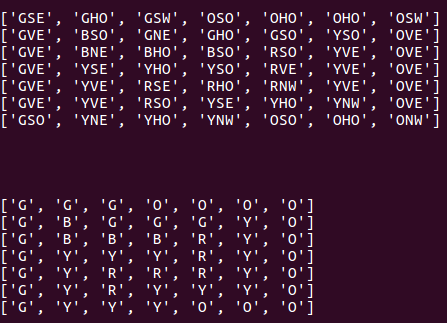
\includegraphics[scale=0.4]{part1/input77.png}
\end{center}
\captionof{figure}{Solution for the 7x7 input. The bottom grid displays the color assignment, while the top grip displays both the color assignment as well as the block type assignment, where 'SO', 'VE', 'HO', 'NE', NW', 'SW', 'SE' refer to block types source, vertical, horizontal, north east, north west, south west, south east, respectively. EG vertical block type has open ends above and below it.}
\begin{center}
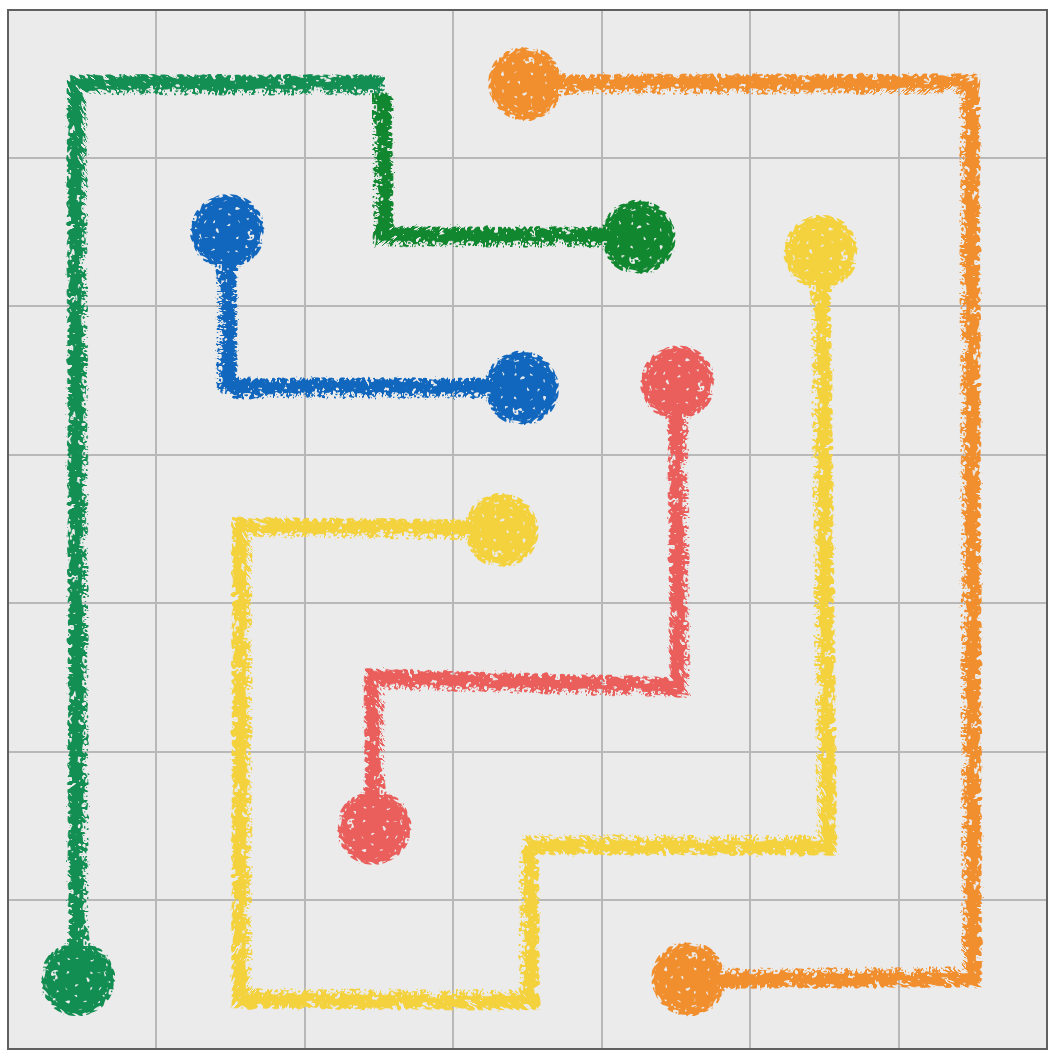
\includegraphics[scale=0.6]{part1/7x7.png}
\end{center}
\captionof{figure}{Visualization of the result for the 7x7 puzzle}

\pagebreak



\subsection*{8x8 Input}
\begin{center}
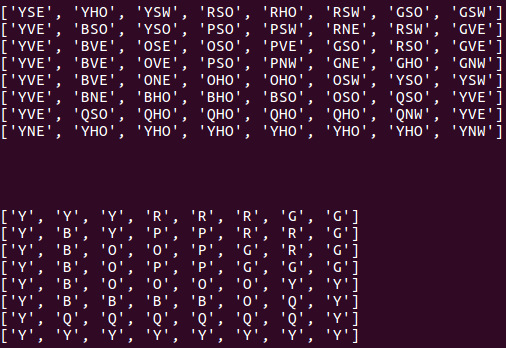
\includegraphics[scale=0.6]{part1/input88.png}
\end{center}
\captionof{figure}{Solution for the 8x8 input. The bottom grid displays the color assignment, while the top grip displays both the color assignment as well as the block type assignment. Please refer to figure 1 description for block type description in the context of solutions.}
\begin{center}
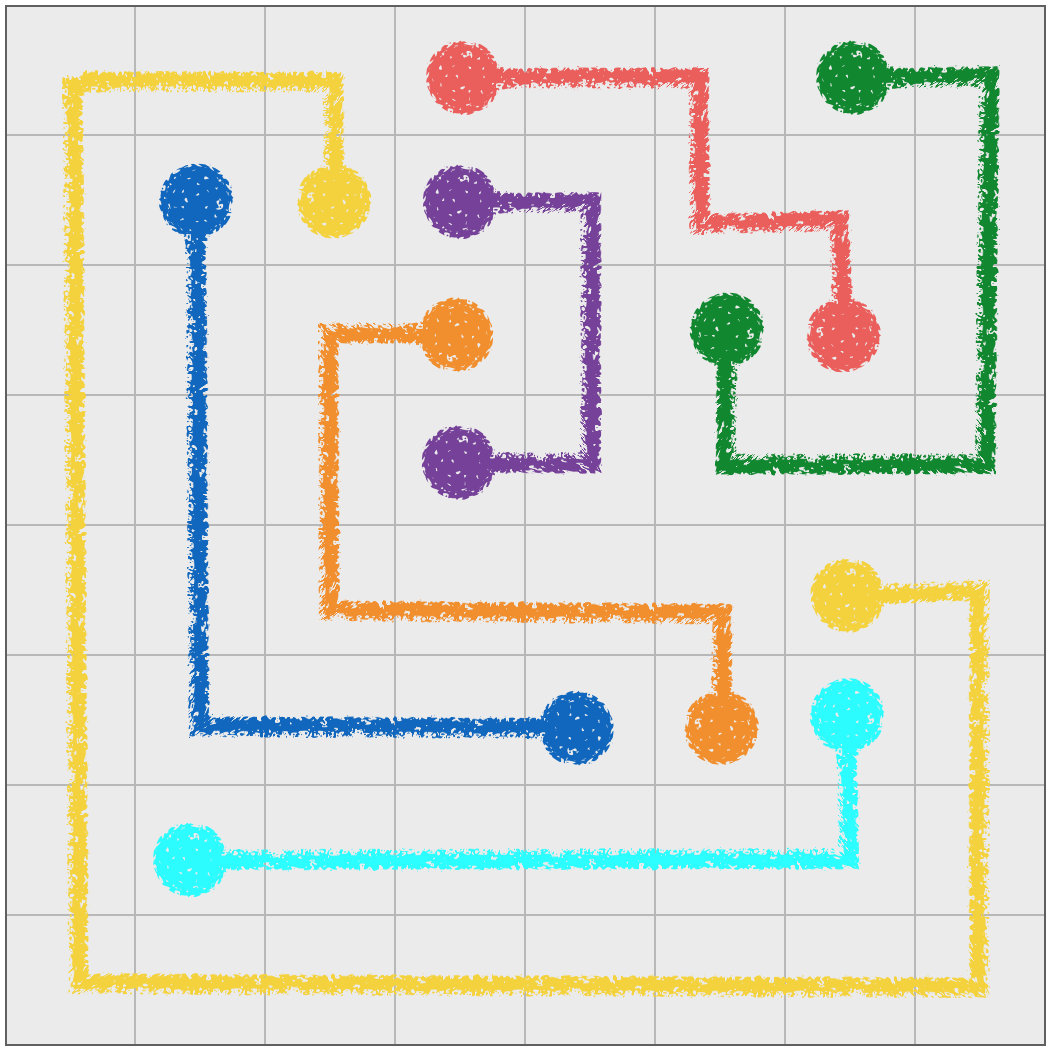
\includegraphics[scale=0.5]{part1/8x8.png}
\end{center}
\captionof{figure}{Visualization of the result for the 8x8 puzzle}


\subsection*{9x9 Input}
\begin{center}
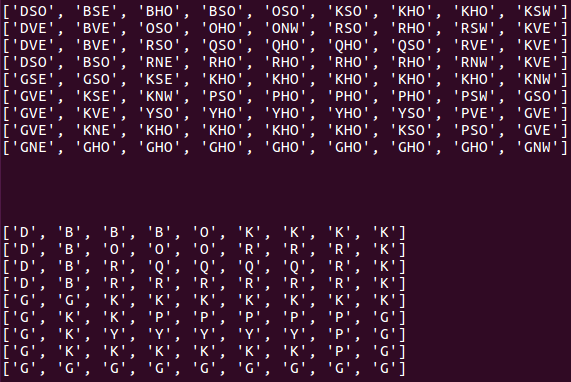
\includegraphics[scale=0.6]{part1/input99.png}
\end{center}
\captionof{figure}{Solution for the 9x9 input. The bottom grid displays the color assignment, while the top grip displays both the color assignment as well as the block type assignment. Please refer to figure 1 description for block type description in the context of solutions.}
\begin{center}
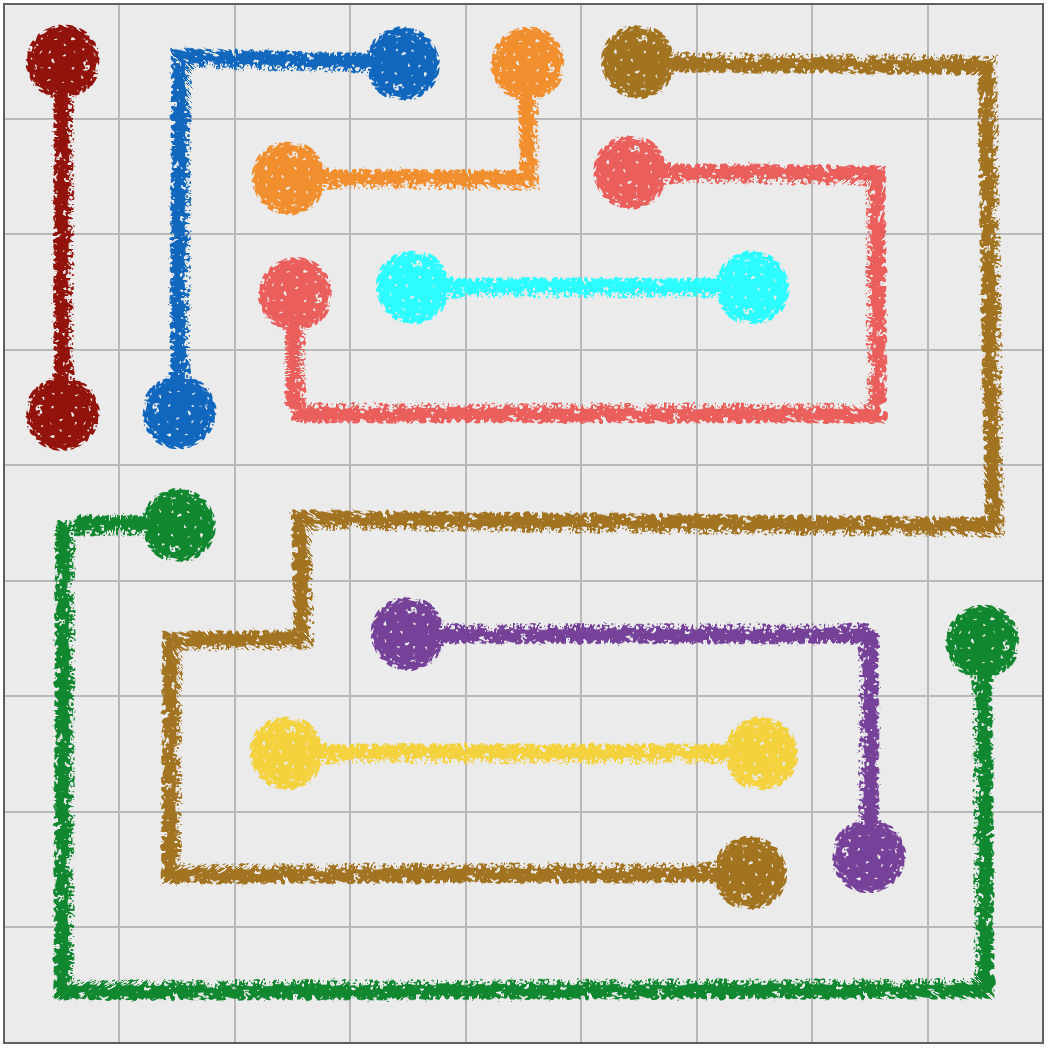
\includegraphics[scale=0.5]{part1/9x9.png}
\end{center}
\captionof{figure}{Visualization of the result for the 9x9 puzzle}
\pagebreak


\subsection*{PART 1.2: Bigger Inputs for Four Credit Students Only}

After completing part 1.1, we added inference in the form of a breadth first search to find connectedness between sources. We added this inference technique to our backtracking solution to achieve the desired 1.2 solutions as shown in figures 7 and 9. Likewise, we show the times for these solutions with the technique in table 1.

This connectedness check is performed where inference is described in the aforementioned base backtracking algorithm. Therefore, once a variable has been assigned a value, we perform a breadth first search over the grid between each pair of sources, where one source is the starting point, and the other is a target. The search can traverse over empty blocks or over blocks with the same color as the same source being searched for. The latter block is acceptable, because the constraints enforce that a pipe based path of that color would be consistent. If a path isn't found between any of the source pairs, then that variable is replaced to be empty, and we backtrack.


\subsection*{PART 1.2: Results}

\subsection*{10x10 (1) Input}
\begin{center}
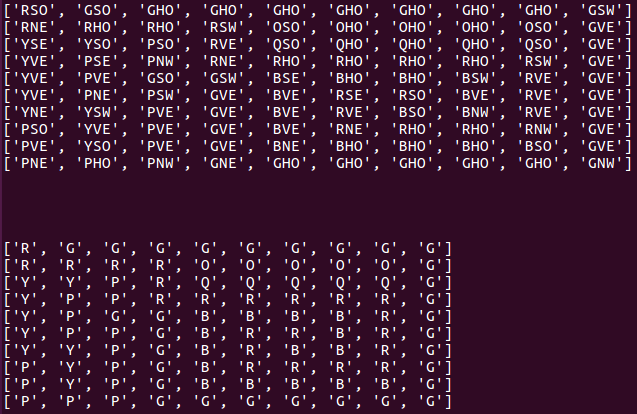
\includegraphics[scale=0.6]{part1/input10101.png}
\end{center}
\captionof{figure}{Solution for the 10x10 (1) input. The bottom grid displays the color assignment, while the top grip displays both the color assignment as well as the block type assignment. Please refer to figure 1 description for block type description in the context of solutions.}
\begin{center}
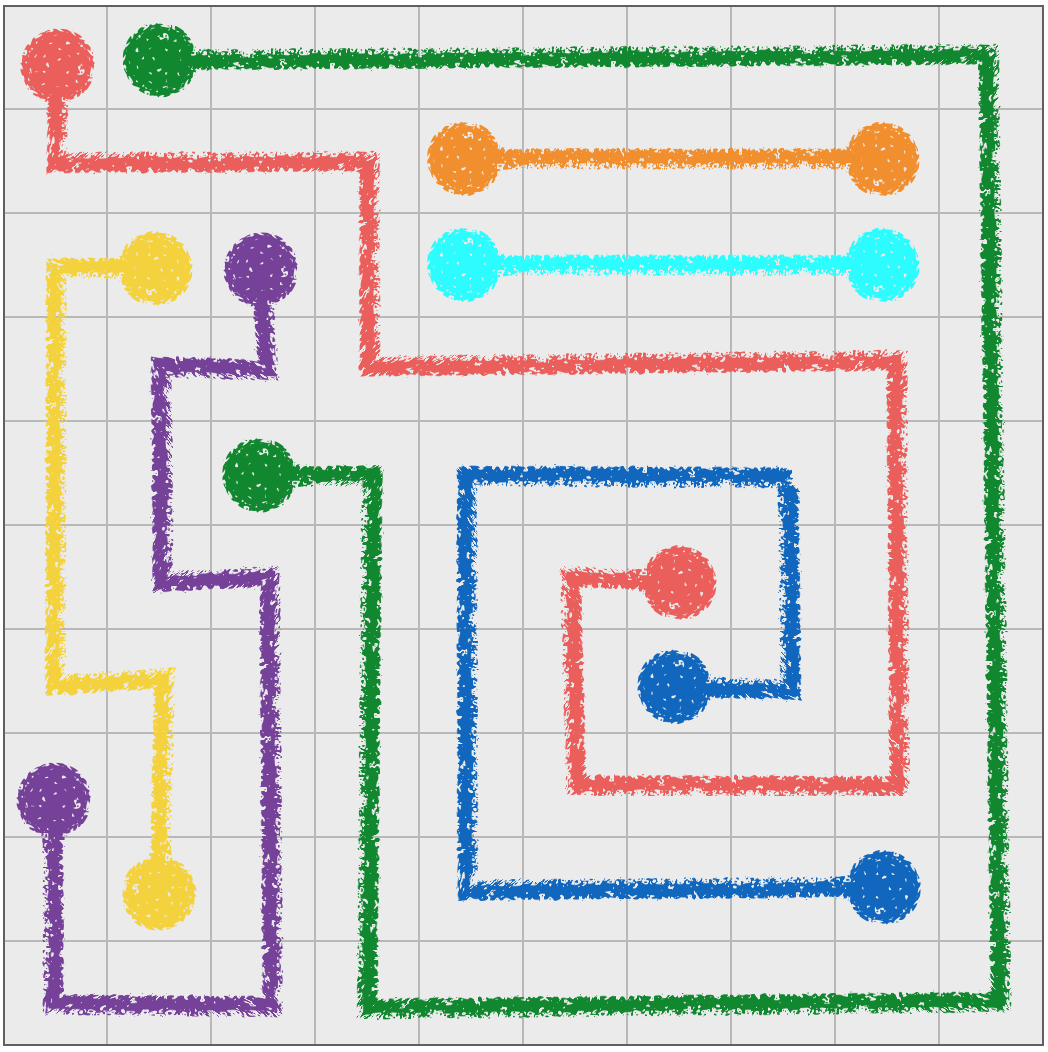
\includegraphics[scale=0.6]{part1/10x10__1_.png}
\end{center}
\captionof{figure}{Visualization of the result for the first 10x10 puzzle}
\pagebreak


\subsection*{10x10 (2) Input}
\begin{center}
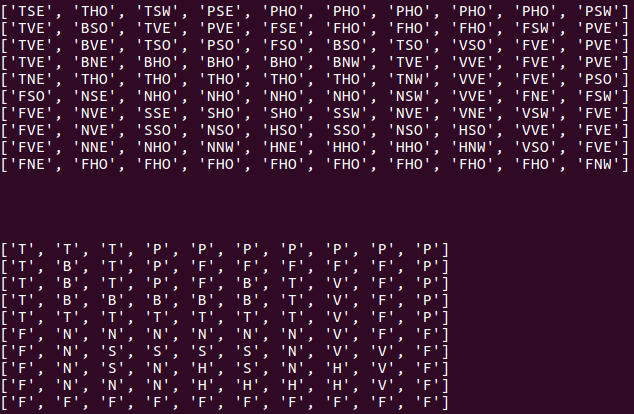
\includegraphics[scale=0.6]{part1/input10102.png}
\end{center}
\captionof{figure}{Solution for the 10x10 (2) input. The bottom grid displays the color assignment, while the top grip displays both the color assignment as well as the block type assignment. Please refer to figure 1 description for block type description in the context of solutions.}
\begin{center}
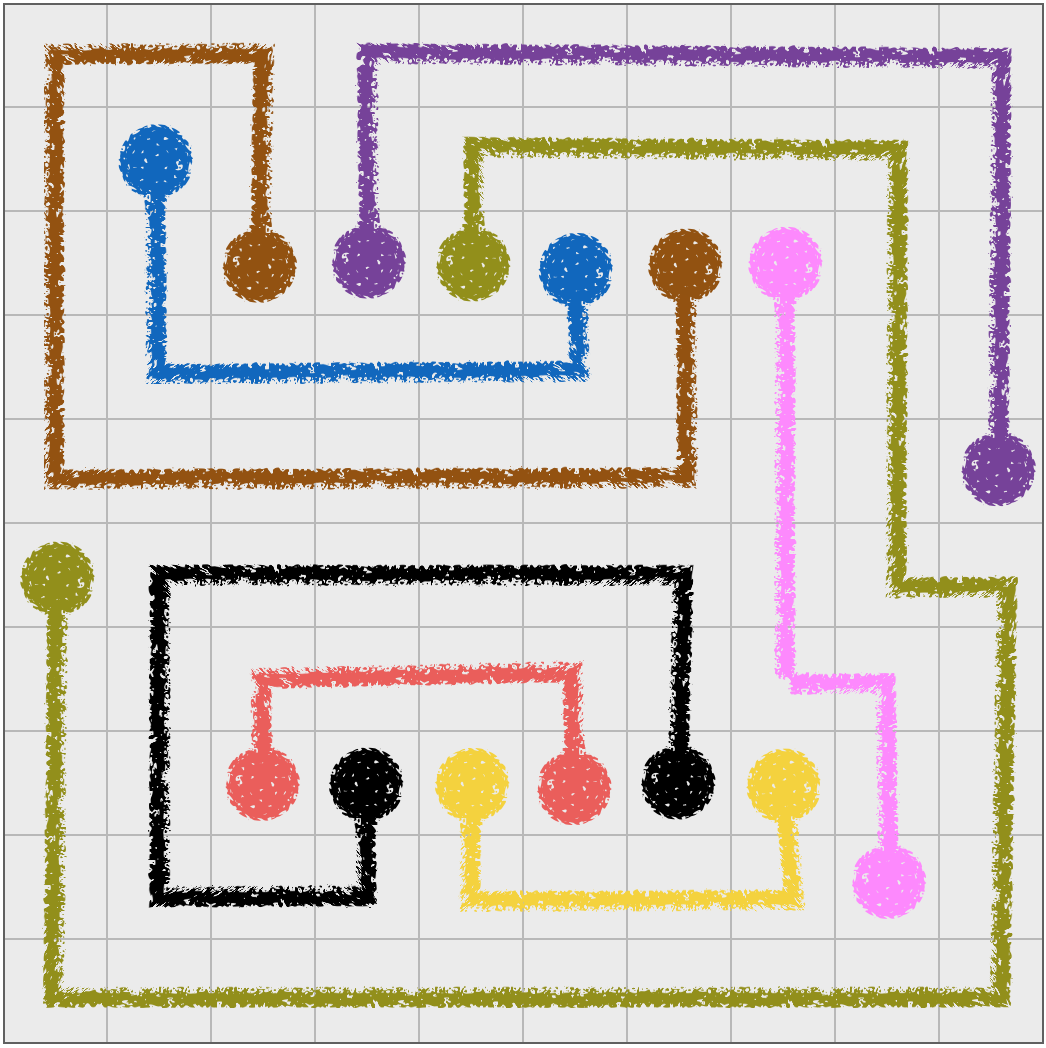
\includegraphics[scale=0.6]{part1/10x10__2_.png}
\end{center}
\captionof{figure}{Visualization of the result for the second 10x10 puzzle}
\pagebreak



\subsection*{Final Results}:\\

\begin{center}
 \begin{tabular}{||c c c c c c||}
 \hline
 input & dumb & MCV & LCV & BFSF & MCValue\\ [0.5ex]
 \hline\hline
 7x7 & N/A & 1163, 0.35 & 846, 0.94 & 285, 0.51 & 138, 0.29\\
 \hline
 8x8 & N/A & 3236, 0.96 & 2675, 3.37 & 1088, 1.94 & 110, 0.31\\
 \hline
 9x9 & N/A & 10695, 3.91 & 16368, 30.13 & 6774, 16.86 & 838, 2.35\\
 \hline
 10x10 (1) & N/A & 500153, 169.37 & N/A & 29975, 74.98  & 2163, 4.72\\
 \hline
 10x10 (2) & N/A & 565664, 196.61 & 135133, 248.43 & 36464, 98.18 & 129014, 350.91 \\ [1ex]
 \hline
\end{tabular}
\end{center}

\captionof{table}{Number of variables assigned and execution time (seconds) for each of the aforementioned backtracking variants including dumb (randomized with no inference); most constrained variable (MCV); least constraining value (LCV); BFS Path Finder; most constraining value (MCValue). N/A refers to when a particular combination of heuristics and inference has an execution time which was too large, and was cut short. Each column describes a heuristic or inference technique. Columns to the right make use of the techniques used in columns to the left such that BFS Path Finder column is using MCV and LCV during its execution. The two exceptions to this are the dumb column, which is incrementally replaced by techniques to the right, and the MCValue column, which uses most constraining value technique in place of the LCV column, which uses the least constraining value technique, but otherwise uses MCV and BFS Path Finder.}

From table 1, some conclusions and insight can be derived. As additional heuristics and inference techniques are added, the performance of backtracking usually improves. However, we see that this isn't the case for the 9x9 and 10x10 (1) input, and that LCV actually reduces the performance of backtracking. It is our hypothesis that this occurs due to the disjoint area of the 9x9 and 10x10 (1) input grid. Least constraining value may allow for a very large branching factor to occur in one of the two areas for that input, but in reality that additional branching factor may not actually help solve the maze as is indicated by its performance. Similarly, most constraining value works well except for 10102 because they are wide open and thus a smaller branching factor is optimal for pruning out options which may lead to less impacted pathways, or in other words, pathways which go into an open area as opposed to traversing the outskirts of the grid. This theory would provide a reasonable explanation for the exception being 10102, since the grid for that requires multiple paths to take a centralized route.


Aside from this conclusion, we can also see that BFS path finding technique significantly improves the performance for all inputs. This indicates that there are a large amount of branches where a solution is impossible due to a lack of connectedness between sources, which this inference procedure accounts for. Of course, for all of these techniques, there is a trade off between computation and branch reduction, but overall it seems that branching contributes more to the execution time than heuristic or inference computation.\\

Finally, it is worth noting that we tried to solve the extra credit puzzles but we couldn't solve any of them in a reasonable amount of time. We performed some profiling on our code to try to understand where the time was being spent and this is what we obtained when finding the solution for the second 10x10 puzzle:
\begin{center}
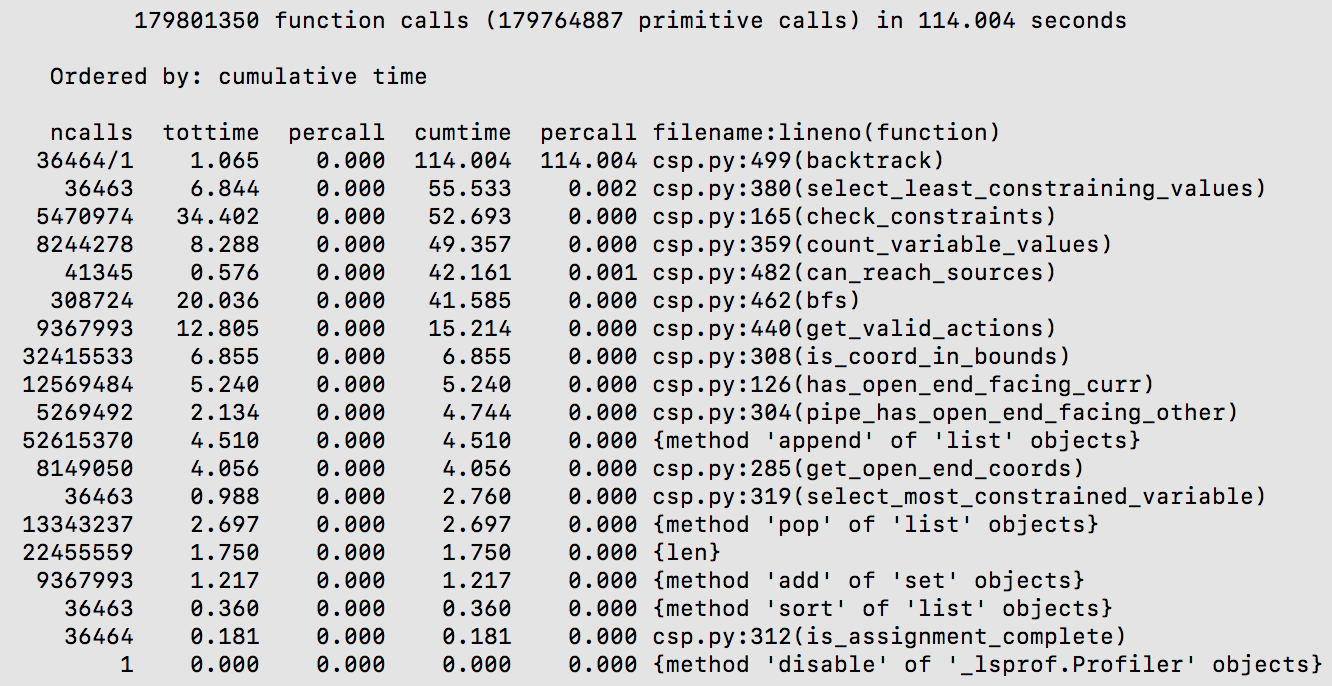
\includegraphics[scale=0.6]{part1/profile.png}
\end{center}
\captionof{figure}{Profiling of the result for the second 10x10 puzzle}

Note that the two most expensive operations are the actual backtracking and \textit{bfs}. Based on that, we think that the only way to solve larger puzzles is by parallelizing some of the work done, potentially the exploration of different branches. If time permits, we will explore this hypothesis.\\

\begin{center}
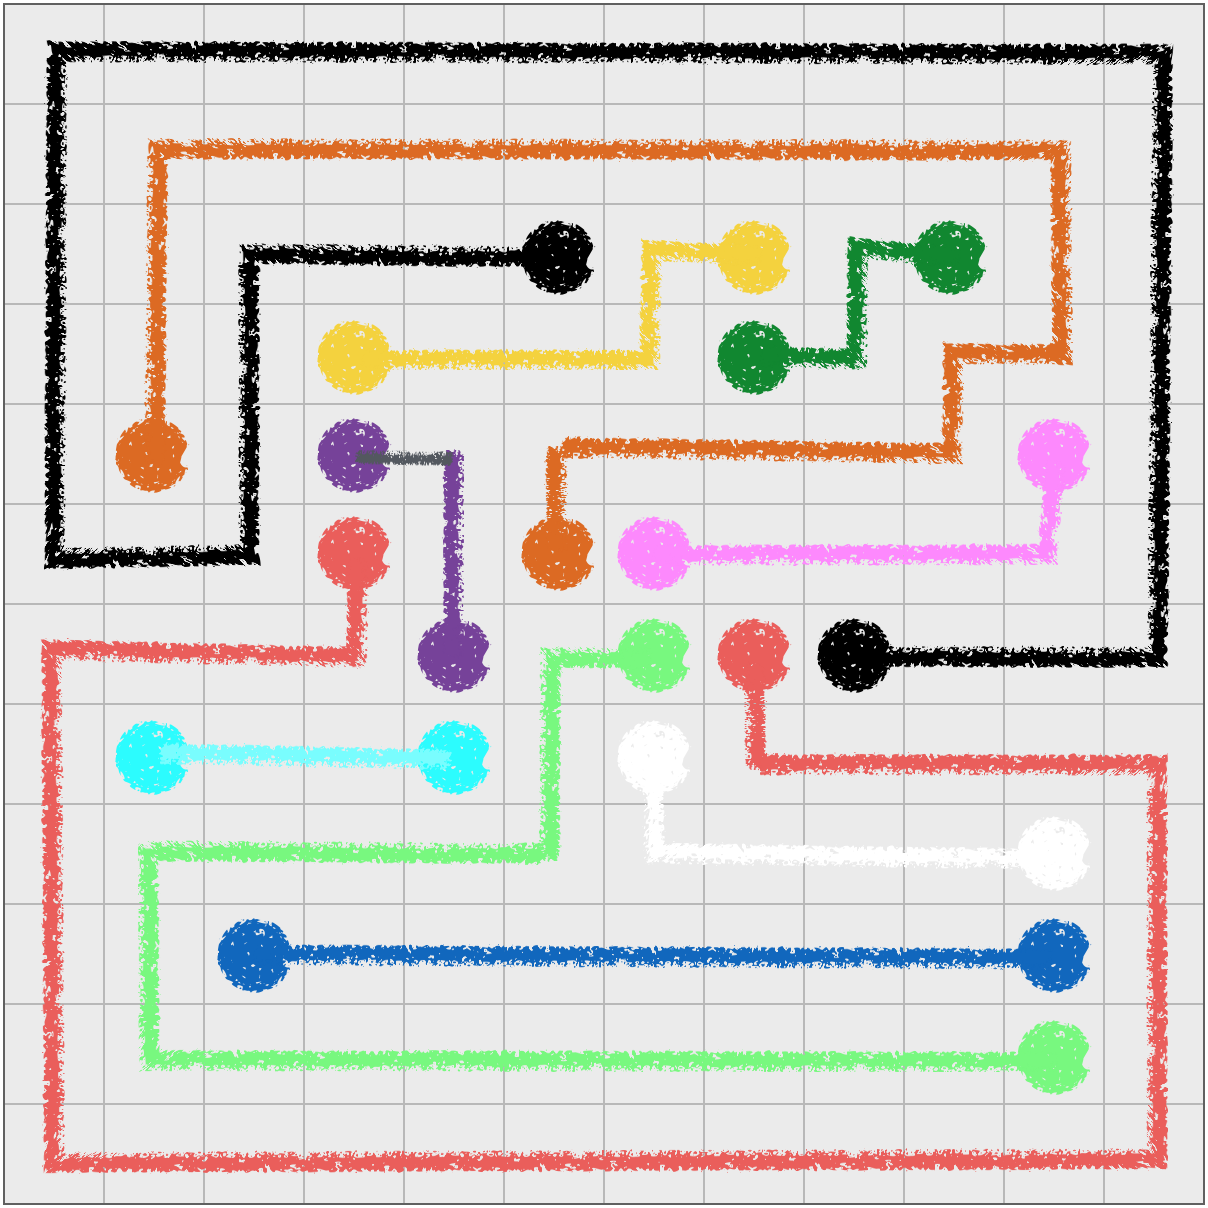
\includegraphics[scale=0.6]{part1/12x12.png}
\end{center}
\captionof{figure}{Visualization of the result for the 12x12 puzzle. Solved by hand.}

It took Nestor roughly 10 minutes to solve the 12x12 puzzle and yet our solver couldn't find a solution after letting it run for at least 40 minutes. What an amazing thing the brain is; we are sure a computer can solve it faster given the right heuristics, heuristics that comes naturally to mind but are hard to tell a computer how to do.

\subsubsection*{Bonus points}
The nice visualizations for the outputs in the previous section are submitted with a request for bonus points, as stated in the homework description.

\pagebreak


\pagebreak
\section*{Part 2: Breakthrough}
Just like in the previous assignment we will use bitmaps to represent the state of the board. Having two bitmaps, one per player, of size equals to the size of the board. A value of 1 indicates that the piece of that player is in a given position.\\

We implemented a \textbf{Game} class inspired in the code for the textbook\footnote{\url{https://github.com/aimacode/aima-python}}. The class is a simple empty skeleton that specifies which methods a game must implement. We then implemented a \textbf{Breakthrough} class that extends \textbf{Game} and implements all its methods. There is a function to generate all the possible actions for a given player given the current state of the board and, more importantly, there is a function that determines when a state is terminal. The \textbf{Breakthrough} class can handle any board size and we use it for the extended rule of using a rectangular board.\\

For the game with the extended rule to take 3 workers home we created a new class called \textbf{Breakthrough3WorkersToBase} which inherits everything from the previous \textbf{Breakthrough} class but overrides the \textit{terminal\_test} function.\\

From now on whenever we may refer to the \textit{state} as the \textit{board} and vice versa. Note that the board has been implemented as a class called \textbf{BreakthroughBoard} and it is responsible of actually moving the pieces/capturing based on an original and final position.


\subsubsection*{Heuristic}
All the heuristic functions can be found under the \textbf{Heuristics} class. Each of the methods is expected to receive two arguments, the first one is the game instance and the second one is the current state. \\

The implementation of the two given heuristics is rather simple. For \textbf{Defensive 1} we simply count how many ones are in the corresponding bitmap of our state representation. Once we have the count we just apply the formula provided. The same goes for \textbf{Offensive 1} with the only difference that you need to look at the other bitmap. \\

For \textbf{Defensive 2} we implemented a weighted function that considers these features of the board:
\begin{enumerate}
\item number of protected cells (both ours and the opponent's): this is the number of cells that can be reached from one of the pieces in a single move and that are not occupied by another piece.
\item row formations: this is when at least two pieces are next to each other.
\item delta formations: this is when a given piece has two pieces diagonally behind it.
\item base cells: how many pieces are still in their base. We value this because they are our last line of defense.
\end{enumerate}

We played a little bit with the weight of each of the features and we ended up with the best results when:
\begin{enumerate}
\item the score is punished for each unprotected cell. An unprotected cell is one that is under attack by the opponent but is it defended by one of your own pieces. For each of those cells we reduce our score by 100.
\item for each of the delta formations we add 75 points to our board score and reduce 75 for each enemy delta formation. We value these formations this high because if a piece is captured we can always retaliate.
\item protected cells add 65 points each. Cells protected by the enemy reduces 65 points.
\end{enumerate}

Besides those features we also check for pieces that are about to win, on both sides, and add or subtract from the score accordingly.\\

For \textbf{Offensive 2} we also implemented a weighted function of features. These are the features:
\begin{enumerate}
\item proximity to the goal: how far into the enemy territory a piece is.
\item arrow formations: created by a piece and all the cells behind it being occupied by friendly pieces.
\item almost win position: increase or decrease the score if board can be won/lost on the next move.
\end{enumerate}

Just like for \textbf{Defensive 2} we played with the weights and settled with:
\begin{enumerate}
\item proximity: 5 points for each row closer to the goal
\item arrow formation: 20 points
\item almost win/lose: 1000 points
\end{enumerate}

\subsubsection*{Analysis}
Why \textbf{Defensive 2} works?\\
Our heuristic emphasizes coverage of the board and delta formations; since \textbf{Offensive 1} only depends on the remaining enemy pieces it is expected that it will try to capture whenever possible. This will immediately be punished if there is a delta formation unless it is about to win. Also, since we value protected cells, we will have more opportunities to capture a piece if it treating us.\\

Why \textbf{Offensive 2} works?\\
Note that our heuristic does not weight in the number of pieces on either side, this offensive strategy relies to getting as far without necessarily capturing pieces, this should allow us to reduce the chance of triggering a response from \textbf{Defensive 1}.\\

\subsubsection*{Results 2.1}
For each of the match-ups requested we played the game four times. The averages are shown below but the results for the individual match-ups can be found in the summary spreadsheet delivered with this report and also online\footnote{\url{https://docs.google.com/a/illinois.edu/spreadsheets/d/1304kvtHACh1N3kYYjGNfJnYtcIc5_p1jHPop4sn356I/edit?usp=sharing}}.\\
In the zip file accompanying this report you will find the whole sequence of moves for every game summarized in this report, as well as the stats for each player. See the \textit{results} directory.\\
Any time measurement is assumed to be in seconds.\\

\textbf{1. Minimax (Offensive 1) vs Alpha-beta (Offensive 1)}\\
Minimax used depth 4 and Alpha-beta used depth 5.
Game results:
\begin{enumerate}
\item Average time per move for whites: \textbf{16.03}
\item Average time per move for blacks: \textbf{0.91}
\item Average \# nodes expanded per move for whites: \textbf{413,445.82}
\item Average \# nodes expanded per move for blacks:  \textbf{21,177.43}
\item Total \# nodes expanded by whites: \textbf{2,796,884.5}
\item Total \# nodes expanded by blacks: \textbf{143,064}
\item Total \# of moves: \textbf{13.5}
\item White pieces captured: \textbf{0.25}
\item Black pieces captured: \textbf{1.5}
\item Winner: Whites
\end{enumerate}
\begin{center}
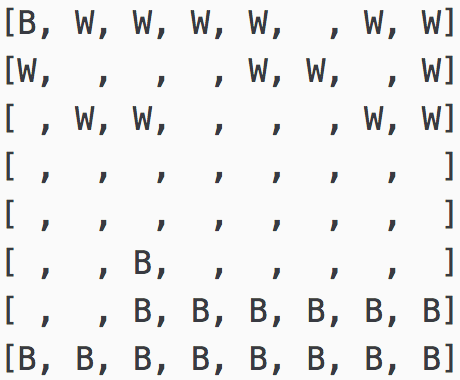
\includegraphics[scale=1]{part2/minimax-o1-vs-ab-o1.png}\\
Final state of the board.
\end{center}
Trends: in all the games the Alpha-beta player won. Which makes since it can see one more move ahead. \\

\pagebreak
\textbf{2. Alpha-beta (Offensive 2) vs Alpha-beta (Defensive 1)}\\
This was run with depth of 4 for both players.\\
Game results:\\
\begin{enumerate}
\item Average time per move for whites: \textbf{0.66}
\item Average time per move for blacks: \textbf{0.25}
\item Average \# nodes expanded per move for whites: \textbf{7,544.1}
\item Average \# nodes expanded per move for blacks:  \textbf{4,403.9}
\item Total \# nodes expanded by whites: \textbf{189,886.75}
\item Total \# nodes expanded by blacks: \textbf{102,276.5}
\item Total \# of moves: \textbf{49.5}
\item White pieces captured: \textbf{0}
\item Black pieces captured: \textbf{2.75}
\item Winner: Whites
\end{enumerate}
\begin{center}
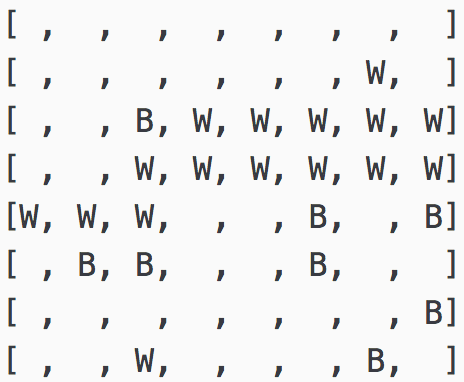
\includegraphics[scale=1]{part2/ab-o2-vs-ab-d1.png}\\
Final state of the board.
\end{center}
Trends: Our heuristic won 3 out of the 4 games played. It was nice to see that the formation that we intended to see in the board actually appeared. Here is an example: \\
\begin{center}
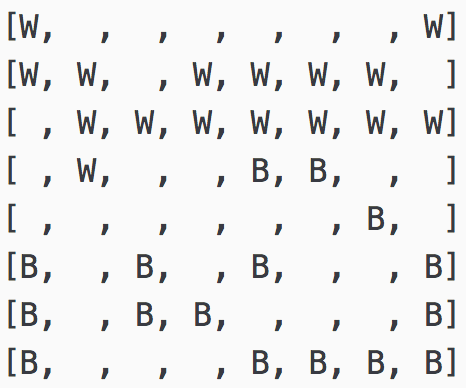
\includegraphics[scale=1]{part2/ab-o2-vs-ab-d1-pattern.png}
\end{center}
See how the white pieces advance but don't try to go on their own and always have "backup".\\

\pagebreak
\textbf{3. Alpha-beta (Defensive 2) vs Alpha-beta (Offensive 1)}\\
This was run with depth of 4 for both players.\\
Game results:\\
\begin{enumerate}
\item Average time per move for whites: \textbf{55.39}
\item Average time per move for blacks: \textbf{3.34}
\item Average \# nodes expanded per move for whites: \textbf{10,067.28}
\item Average \# nodes expanded per move for blacks:  \textbf{2,514.29}
\item Total \# nodes expanded by whites: \textbf{160,601.75}
\item Total \# nodes expanded by blacks: \textbf{45,653.75}
\item Total \# of moves: \textbf{36}
\item White pieces captured: \textbf{0}
\item Black pieces captured: \textbf{2}
\item Winner: Whites
\end{enumerate}
\begin{center}
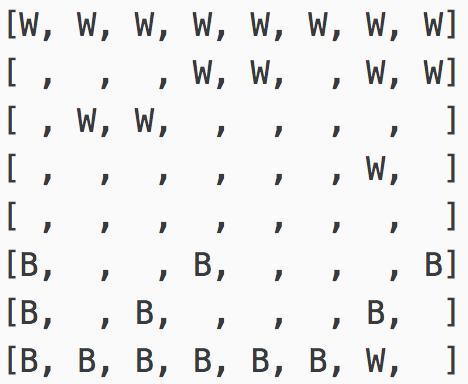
\includegraphics[scale=1]{part2/ab-d2-vs-ab-o1.png}\\
Final state of the board.
\end{center}
Trends: Our heuristic won 4 out of the 4 games played. The delta formations we were expecting to see showed up most of the times. Here is an example: \\
\begin{center}
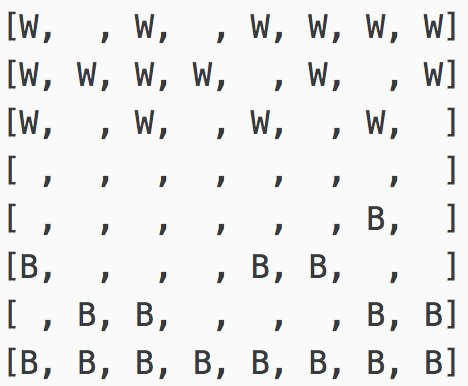
\includegraphics[scale=1]{part2/ab-d2-vs-ab-o1-pattern.png}
\end{center}
We realize this formation would be bad for a smarter opponent (and it is confirmed later on in this report) because of the "holes" in the delta formation but it turns out to work well against the provided defensive heuristic.\\

One thing to note is that for this match-up the second game took way longer than the other games. Time between moves was around 2 minutes. Our only guess is that it was caused by the fact that we were running a script for our data mining course at the same time. We could never replicate it after that.\\

\pagebreak
\textbf{4. Alpha-beta (Offensive 2) vs Alpha-beta (Offensive 1)}\\
This was run with depth of 4 for both players.\\
Game results:\\
\begin{enumerate}
\item Average time per move for whites: \textbf{0.51}
\item Average time per move for blacks: \textbf{0.17}
\item Average \# nodes expanded per move for whites: \textbf{6,463.52}
\item Average \# nodes expanded per move for blacks:  \textbf{3,183.71}
\item Total \# nodes expanded by whites: \textbf{197,461.5}
\item Total \# nodes expanded by blacks: \textbf{95,030.75}
\item Total \# of moves: \textbf{60.25}
\item White pieces captured: \textbf{0.25}
\item Black pieces captured: \textbf{4.75}
\item Winner: Whites
\end{enumerate}
\begin{center}
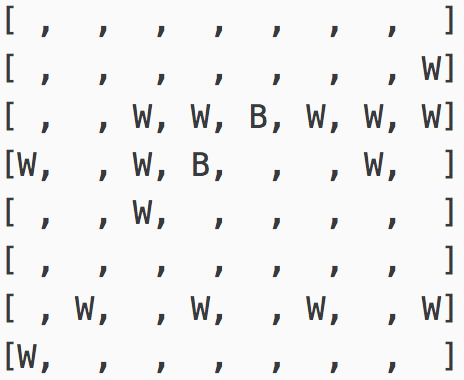
\includegraphics[scale=1]{part2/ab-o2-vs-ab-o1.png}\\
Final state of the board.
\end{center}
Trends: at first we didn't expect \textbf{Offensive 2} to beat \textbf{Offensive 1} but after looking at the results it does make sense. The reason is that almost always when \textbf{Offensive 1} would take a piece the opponent would have a way to respond because of the value we gave to "moving as a front". As a result of this, this match-up has the highest number of pieces captured on average.\\

\pagebreak
\textbf{5. Alpha-beta (Defensive 2) vs Alpha-beta (Defensive 1)}\\
This was run with depth of 4 for both players.\\
Game results:\\
\begin{enumerate}
\item Average time per move for whites: \textbf{1}
\item Average time per move for blacks: \textbf{0.22}
\item Average \# nodes expanded per move for whites: \textbf{6,111.88}
\item Average \# nodes expanded per move for blacks:  \textbf{3,524.07}
\item Total \# nodes expanded by whites: \textbf{136,086.25}
\item Total \# nodes expanded by blacks: \textbf{69,990.5}
\item Total \# of moves: \textbf{41.5}
\item White pieces captured: \textbf{0}
\item Black pieces captured: \textbf{2}
\item Winner: Whites
\end{enumerate}
\begin{center}
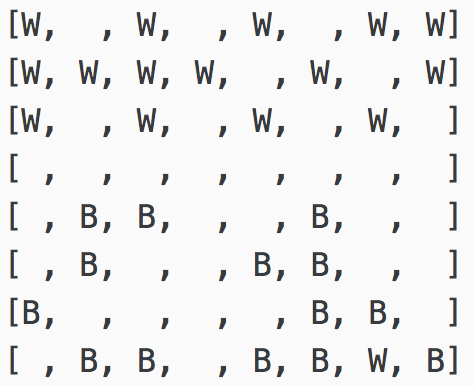
\includegraphics[scale=1]{part2/ab-d2-vs-ab-d1.png}\\
Final state of the board.
\end{center}
Trends: It makes sense for heuristic \textbf{Defensive 2} to beat \textbf{Defensive 1} because our heuristic still considers the value of the pieces as \textbf{Defensive 1} does but it also considers other features of the board.\\

\pagebreak
\textbf{6. Alpha-beta (Offensive 2) vs Alpha-beta (Defensive 2)}\\
This was run with depth of 4 for both players.\\
Game results:\\
\begin{enumerate}
\item Average time per move for whites: \textbf{0.41}
\item Average time per move for blacks: \textbf{0.22}
\item Average \# nodes expanded per move for whites: \textbf{6,010.24}
\item Average \# nodes expanded per move for blacks:  \textbf{1,680.6}
\item Total \# nodes expanded by whites: \textbf{294,502}
\item Total \# nodes expanded by blacks: \textbf{80,669}
\item Total \# of moves: \textbf{97}
\item White pieces captured: \textbf{1}
\item Black pieces captured: \textbf{14}
\item Winner: Whites
\end{enumerate}
\begin{center}
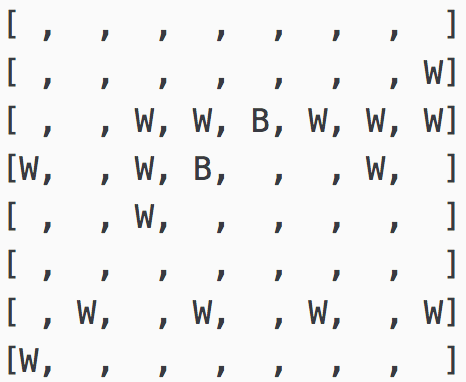
\includegraphics[scale=1]{part2/ab-o2-vs-ab-d2.png}\\
Final state of the board.
\end{center}
Trends: as mentioned earlier, \textbf{Defensive 2} heuristic isn't very smart because the delta formations leave an open path for the enemy.\\
Although we ran the match-up four times, the results were the same. This makes sense because there is no randomness on either side of the board. \\

\subsubsection*{Extended rules}
For part 2.2 we were asked to add additional rules to the board. All the code was written thinking about these extended rules since the beginning so in order to play a match in a 10x5 board the only thing we needed to do was to change the size of the board argument in our \textbf{Breakthrough} class.\\
For the 3 workers to base rule we created a new class (\textbf{Breakthrough3WorkersToBase}) that extends the normal \textbf{Breakthrough} class and overrides the \textit{terminal\_test} method. This new method checks for two things: number of pieces in the base row is 3 or remaining pieces is 2 (can't win).\\
Note that we didn't have to change the evaluation function because we designed it from the beginning to consider multiple pieces at base in the weighted function and it also depends on the number of pieces, which will change based on the size of the board (for the rectangular board for instance).

Lets look at the results.\\

\subsubsection*{Results 2.2}

\textbf{1. 3 workers to base}\\
We decided to use \textbf{Offensive 1} and \textbf{Defensive 1} for the match-ups.\\

The games were run with depth of 5 for both players.\\
Game results:\\
\begin{enumerate}
\item Average time per move for whites: \textbf{3.21}
\item Average time per move for blacks: \textbf{3.1}
\item Average \# nodes expanded per move for whites: \textbf{83,946.52}
\item Average \# nodes expanded per move for blacks:  \textbf{70,858.69}
\item Total \# nodes expanded by whites: \textbf{3,938,242.75}
\item Total \# nodes expanded by blacks: \textbf{3,304,344.7}
\item Total \# of moves: \textbf{94.75}
\item White pieces captured: \textbf{7.75}
\item Black pieces captured: \textbf{9}
\item Winner: Blacks (3 out of 4 times)
\end{enumerate}
\begin{center}
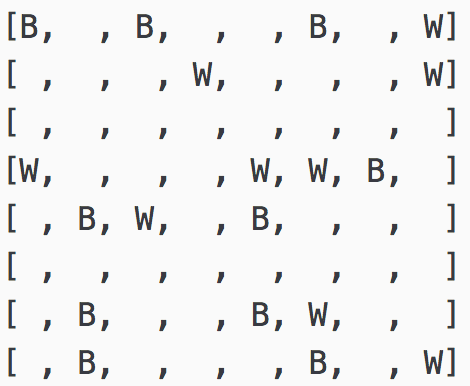
\includegraphics[scale=1]{part2/ab-o1-vs-ab-d1-3workers-black.png}\\
Game won by 3 pieces at the base.\\

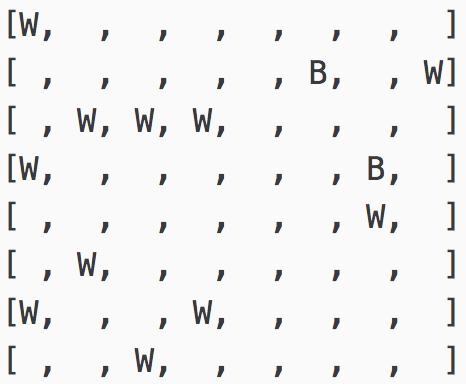
\includegraphics[scale=1]{part2/ab-o1-vs-ab-d1-3workers-whites.png}\\
Game won by 3 pieces at the base.\\
\end{center}
One of the interesting things about this setup is that the only time Whites won was because they captured all black pieces not because they took 3 pieces to base. In contrast, all the games won by Blacks were won by taking 3 pieces to base and not by capturing all white pieces. In all cases, it seems like the player that captured the most pieces wins.\\

\textbf{2. Rectangular board}\\
There was some discrepancy between what the professor said about the 5x10 board (10 pieces on each side) and what the TA said (20 pieces on each); just to be sure that we don't lose points because of that, we present both results.\\

The games were run with depth of 5 for both players.\\

Game results:\\
\begin{enumerate}
\item Average time per move for whites: \textbf{3.08}
\item Average time per move for blacks: \textbf{1.02}
\item Average \# nodes expanded per move for whites: \textbf{79,968.26}
\item Average \# nodes expanded per move for blacks:  \textbf{24,608.09}
\item Total \# nodes expanded by whites: \textbf{1,329,205}
\item Total \# nodes expanded by blacks: \textbf{317,786.25}
\item Total \# of moves: \textbf{38.75}
\item White pieces captured: \textbf{4.5}
\item Black pieces captured: \textbf{14}
\item Winner: Whites (3 out of 4 times)
\end{enumerate}
\begin{center}
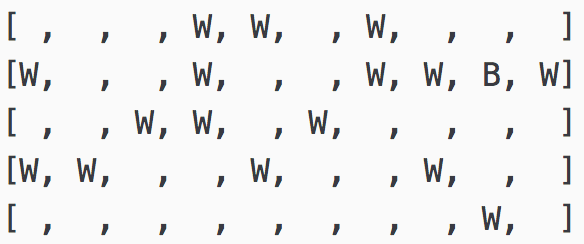
\includegraphics[scale=1]{part2/ab-01-vs-ab-d1-rect5x10.png}\\
Final state of the board for one of the matches.
\end{center}
The interesting thing about this board is that it caused the players to "think more", pretty much all the metrics are higher in this board than in the 5x10 board (shown below). This may be simply due to the fact that there are twice as many pieces which means that the number of actions at each move is higher.\\

We also ran some games in a rectangular 10x5 (as opposed to 5x10). The results were this:
\begin{enumerate}
\item Average time per move for whites: \textbf{0.86}
\item Average time per move for blacks: \textbf{0.58}
\item Average \# nodes expanded per move for whites: \textbf{23,419.22}
\item Average \# nodes expanded per move for blacks:  \textbf{14,520.39}
\item Total \# nodes expanded by whites: \textbf{760,800.25}
\item Total \# nodes expanded by blacks: \textbf{459,584}
\item Total \# of moves: \textbf{65.5}
\item White pieces captured: \textbf{1.75}
\item Black pieces captured: \textbf{6.25}
\item Winner: Whites
\end{enumerate}
\begin{center}
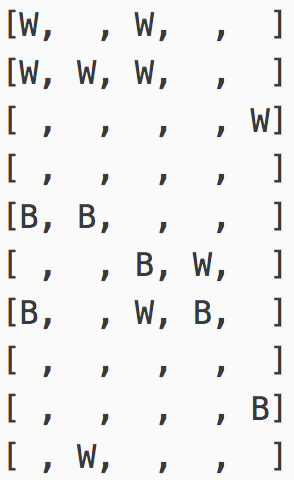
\includegraphics[scale=1]{part2/ab-o1-vs-ab-d1-rect10x5.png}\\
Final state of the board for one of the matches.
\end{center}

\subsubsection*{Final thoughts}
Based on the results, it seems like offensive heuristics perform better. It is hard to tell if this is true in general because the defensive heuristics used here were rather poor: one was designed to be beaten and the other one designed only to beat a particular opponent.\\

Move ordering seems to make a huge impact in the number of nodes expanded, in combination with alpha-beta pruning, of course.

\subsubsection*{Potential Extra Credits}
As you may have noticed the number of expanded nodes for matches between both alpha-beta players are relatively low. We implemented move ordering based on the board configuration at depth 1. We also tried to do the ordering  on each level (inside the min-value and max-value functions) but it was taking too long to finish so we decided to keep it just in the first level.\\

We implemented a multi-feature weighted evaluation function instead of going with the simple evaluation function described in the game's Wikipedia page.\\

We found in the book a method called \textit{beam search} which consists of just cutting off some of the search. It relies on a strong move ordering heuristic. Since our games were not taking too long we decided not to implement it. May be worth it if we increase the depth of the search to a point where we can't tolerate to consider all the actions even with alpha-beta pruning. We will try this if time permits.\\

\subsubsection*{Statement of individual contribution}
Edward worked on Part 1 of the assignment and Nestor worked on Part 2. This includes both the programming and report writing tasks. Discussions and revising of the report involved both of us.

\end{document}
